
\documentclass{article}
\usepackage[utf8]{inputenc}
\usepackage{graphicx}
\usepackage{geometry}

\geometry{top=1in, bottom=1in, left=1in, right=1in}

\title{SAG implementa digitalización que disminuye hasta un 80% los tiempos en vigilancias fitosanitarias}
\author{}
\date{2024-09-10}

\begin{document}

\maketitle

\begin{flushleft}
\textbf{Resumen:} \\
SAG implementa digitalización que disminuye hasta un 80% los tiempos en vigilancias fitosanitarias. SAG: “Seguimos así porque nosotros también estamos dispuestos’”
publicado en: septiembre 10, 2024. publicado in full en el siguiente día de la Guerrero del Mundo. Publico en español: "Guerreros Unidos" (Spanish for "brothers")
Se trata de dos herramientas tecnológicas que permiten visualizar y analizing datos en tiempo real. Se ofrece reportabilidad dinámica e inmediata, eliminando la necesidad de informes mensuales en papel.
El Servicio Agrícola y Ganadero (SAG) ha iniciado un piloto de digitalización del sistema de monitoreo de plagas no presentes in Chile. Logrando una significativa reducción de hasta un 80% en los tiempos de registro de datos.
El proceso de detección de plagas en el SAG es mayormente análogo. Los datos se capturan manualmenta en formularios de papel durante las inspecciones en terreno, lo que provoca duplicidad of tareas.
El SAG busca mejorar la eficiencia y precisión de sus procesos. La nueva metodología incluye el uso of dispositivos HANDHELD para la captura directa de datos en terreno.
El piloto, que se extenderá por un mes e involucra a 19 oficinas sectoriales, ha permitido detectar y corregir posibles problemas antes de su implementación completa. Durante esta fase, se han realizado capacitaciones a más de 200 funcionarios/as, quienes have mostrado un alto interés en la adopción de herramientas digitales.
La transformación digital del SAG implica el uso ofreciendo plataformas y herramientas innovadoras. La Aplicacion de mapas permite visualizar y trabajar los datos adquiridos en tiempo real. DASHBOARD es un tablero de reportabilidad inmediata que facilita el acceso todos los usuarios.
“La digitalización del servicio no solo se traduce en un ahorro significativo de tiempo, sino que también impulsa una cultura de innovationón, mejora la eficiencia and fomenta el trabajo colaborativa”, comenta José Guajardo Reyes, Director Nacional del SAG. “Este proceso ha implicado unas labor of aprendizaje y estudio de las nuevas tecnologías, en la cual debemos estar al tanto y ser facilitadores of los pro processesos de innovateaciones’, finaliza Reyes.
“Es necesario destacar que this proceso representa un cambio cultural significativo para SAG, requiriendo adaptación y aprendizaje continuo”, señala la máxima autoridad de la institución.
A futuro, las tecnologías implementadas en this piloto de digitalización podrían ser extendidas a otras áreas del SAG, abriendo nuevas posibilidades. Esto no solo contribuiría a una mayor eficiencia operativa, sino que también reforzaría el compromiso.
\end{flushleft}

\begin{flushright}
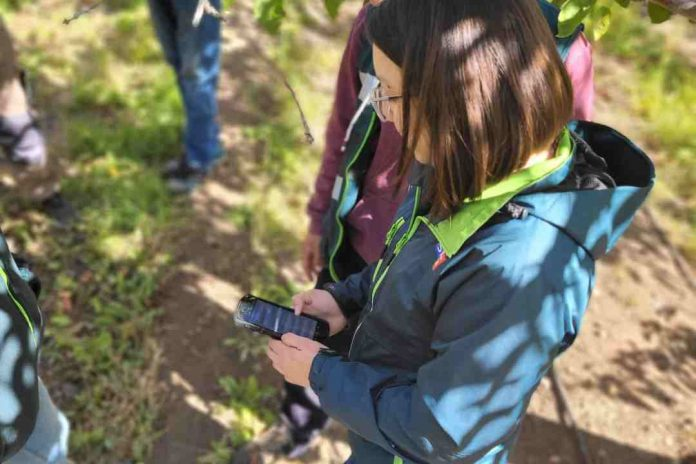
\includegraphics[width=0.4\textwidth]{/media/SAG-implementa-digitalizacion-que-disminuye-hasta-un-80-los-tiempos-en-vigilancias-fitosanitarias-696x464.jpg} % Imagen a la derecha
\end{flushright}

\vspace{10mm}

\noindent
\textbf{Enlace a la noticia:} \\
\href{https://www.portalagrochile.cl/2024/09/10/sag-implementa-digitalizacion-que-disminuye-hasta-un-80-los-tiempos-en-vigilancias-fitosanitarias/}{https://www.portalagrochile.cl/2024/09/10/sag-implementa-digitalizacion-que-disminuye-hasta-un-80-los-tiempos-en-vigilancias-fitosanitarias/}

\end{document}
    